\section{Use cases: given a metabolic model...}
\label{section:use-cases}

La figura \footnote{aggiungere qui una figura che rappresenta gli use
  case in stile overview} riassume tutti i casi d'uso che abbiamo
implementato nella libreria. La notazione utilizzata \`e quella
offerta dal linguaggio \emph{UML}, limitandosi ai "costrutti" pi\`u
semplici per favorire la comprensione.

In questa sezione descriveremo i casi d'uso che vogliamo implementare
e, per ognuno di essi, mostreremo i risultati della realizzazione.

Come suggerisce il titolo di questa sezione, tutti i successivi use
case lavorano su un modello metabolico, sul quale vengono effettuate
le trasformazioni che andiamo a dettagliare. Inoltre, come il lettore
capir\`a tra nelle prossime righe, ogni use case pu\`o essere messo in
corrispondenza con il concetto di filtro. Questa associazione
porter\`a alla naturale astrazione che cosistuir\`a l'architettura
della nostra libreria.

\subsection{...build a model \emph{story-ready}}
L'operazione fondamentale a cui siamo interessati \`e poter manipolare
un modello metabolico, codificandolo con un sistema di oggetti che
permetta di applicare i concetti espressi in \footnote{aggiungere qui
  riferimento bibliografico all'articolo Crescenzi-Marino}.

Questo requisito precede tutti gli altri, in quanto questi suppongono
che il modello che vogliamo studiare sia gi\`a stato codificato nel
nostro modello dati.

Non possiamo dare nessun oggetto che sia la rappresentazione di questo
use case, in quanto la miglior rappresentazione del risultato della
sua esecuzione \`e un insieme di oggetti Java, di cui evitiamo di
riportare la rappresentazione testuale fornita dal metodo
\emph{toString()}.

\subsection{...represent it in \emph{black \& white}}
\label{subsection:represent-it-in-black-and-white}
Questo use case cattura il requisito di costruire un documento
interpretabile dai motori di renderizzazione offerti dalla libreria
\emph{graphviz}, rappresentando i nodi sorgenti e nodi pozzi con un
cerchio completamente riempito (\emph{black nodes}), mentre i nodi che
non sono ne sorgente ne pozzi con un cerchio vuoto (\emph{white
  nodes}).
\begin{figure}
  \centering
  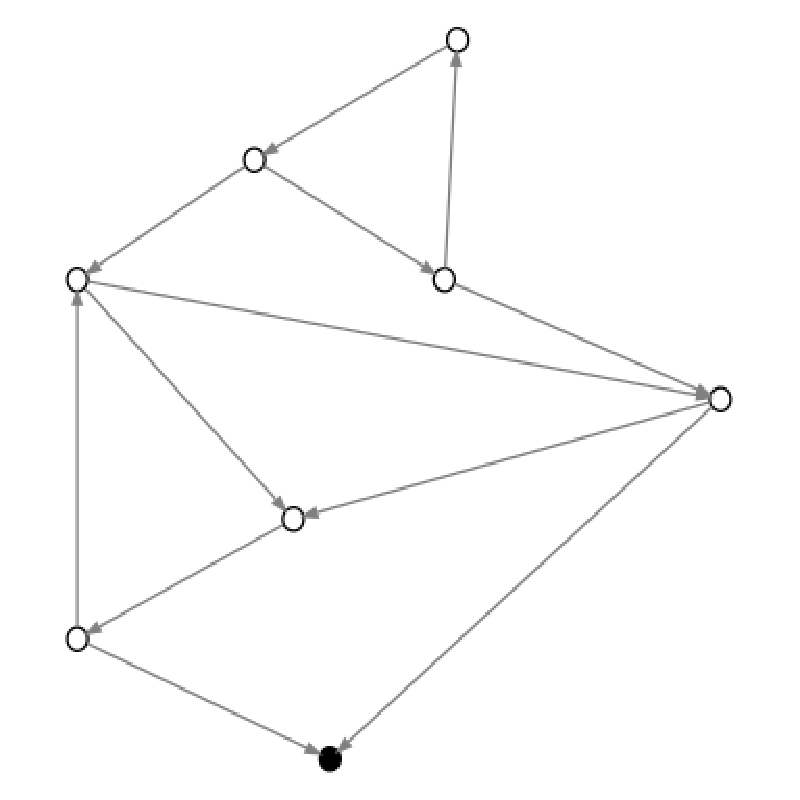
\includegraphics[scale=0.8]{images/applicationOfPrinterPipeFilterOnTarjanModel-phase-PrinterPipeFilter-level-0.eps}
  \caption{simple black \& white graph}
  \label{fig:simple-black-and-white}
\end{figure}

La figura \ref{fig:simple-black-and-white} riporta la rappresentazione
di un modello metabolico dopo esser stato codificato nel nostro
modello dati.

Questo use-case non ha restituisce nessuna trasformazione del grafo in
input, pertanto si limita a restituire il grafo originale.

\subsection{...apply a \emph{DFS search} and build its tree}
Questo use case cattura il requisito di applicare un ricerca
\emph{DFS} al grafo in input.

Il risultato prodotto da questo use-case \`e la foresta di alberi
\emph{DFS}, i cui archi sono un sottoinsieme dell'insieme di archi del
grafo originale visitati durante la computazione.

Inoltre, siamo interessati ad associare, per ogni vertice, una coppia
di interi che indica il momento in cui la visita esplora un vertice e
quando l'esplorazione del vicinato di tale vertice viene
completata. Queste informazioni possono risultare molto utili in fase
di studio del grafo; abbiamo ripreso questo spunto da
\footnote{aggiungere qui riferimento bibliografico a Algorithms}.

Vediamo i risultati di una sua esecuzione: la figura
\ref{fig:before-applying-dfs-search} riporta il grafo originale di
partenza, preso da \footnote{aggiungere qui riferimento bibliografico
  al volume di Papadimitriou Algorithms}:
\begin{figure}
  \centering
  
\includegraphics{images/OnePipingLevelUnitTest_Printer_DFS_PrinterPipe_Papadimitriou-phase-PrinterPipeFilter-level-0.eps}
  \caption{Before applying DFS search}
  \label{fig:before-applying-dfs-search}
\end{figure}
applicando la ricerca \emph{DFS} a tale grafo otteniamo la foresta di
alberi \emph{DFS}, riportata in figura \ref{fig:dfs-forest}, dopo aver
composto a questo use-case il precedente
\ref{subsection:represent-it-in-black-and-white}.
\begin{figure}
  \centering
  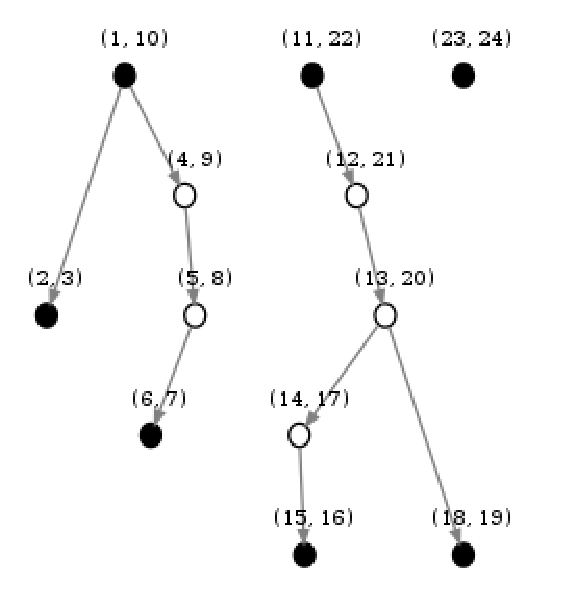
\includegraphics{images/OnePipingLevelUnitTest_Printer_DFS_PrinterPipe_Papadimitriou-phase-PrinterPipeFilter-level-2.eps}
  \caption{DFS forest}
  \label{fig:dfs-forest}
\end{figure}

\subsection{...apply the \emph{Tarjan algorithm} and build the
  minimized graph}
Questo use case cattura il requisito di applicare l'algoritmo di
Tarjan per la ricerca delle componenti fortemente connesse al grafo di
input.

Il risultato prodotto da questo use-case \`e un grafo che ha
come nodi le componenti fortemente connesse e come archi la relazione
di vicinato tra le componenti.

Inoltre, siamo interessati ad associare, per ogni vertice, un intero
che indica la cardinalit\`a della componente fortemente connessa che
esso rappresenta.

Vediamo i risultati di una sua esecuzione: la figura
\ref{fig:before-applying-tarjan} riporta il grafo originale di
partenza, preso da \footnote{aggiungere qui riferimento bibliografico
  al volume di Crescenzi sulle strutture dati}:
\begin{figure}
  \centering
  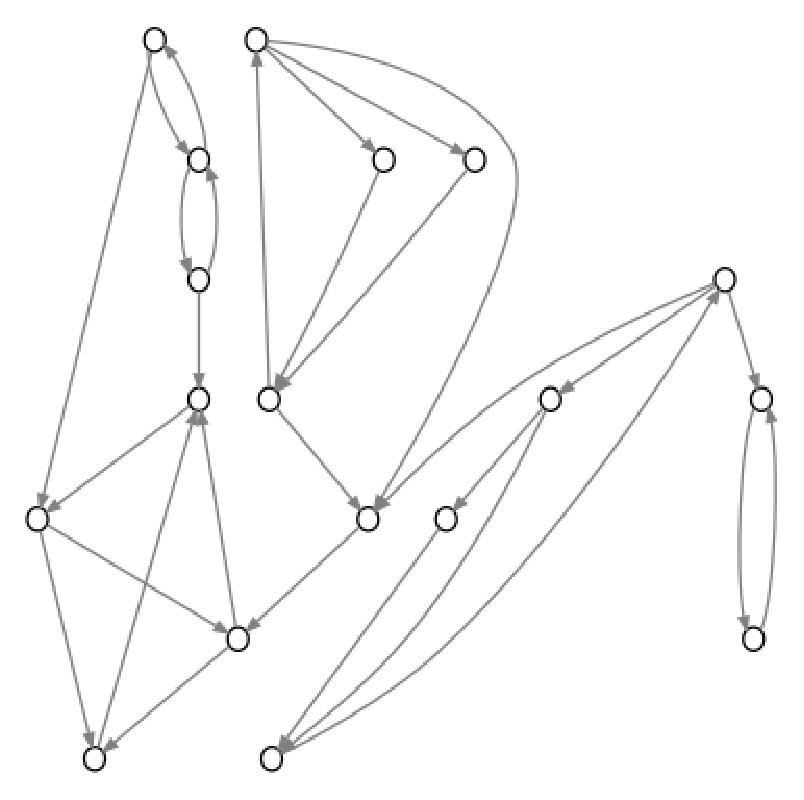
\includegraphics{images/OnePipingLevelUnitTest_Printer_DFS_PrinterPipe_Crescenzi-phase-PrinterPipeFilter-level-0.eps}
  \caption{Before applying Tarjan algorithm}
  \label{fig:before-applying-tarjan}
\end{figure}
applicando l'algoritmo di Tarjan a tale grafo otteniamo il grafo
minimizzato, riportato in figura \ref{fig:tarjan-output}, dopo aver
composto a questo use-case il precedente
\ref{subsection:represent-it-in-black-and-white}.
\begin{figure}
  \centering
  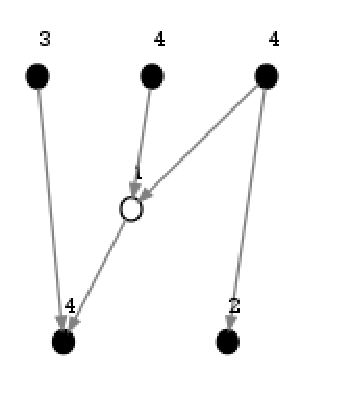
\includegraphics{images/OnePipingLevelUnitTest_Printer_DFS_PrinterPipe_Crescenzi-phase-PrinterPipeFilter-level-2.eps}
  \caption{Graph after Tarjan minimization}
  \label{fig:tarjan-output}
\end{figure}

\subsection{...represent it in \emph{plain text} tabular}

\subsection{...\emph{collapse} its source to manage complexity}

\subsection{...\emph{inspect} its connected components and \emph{show}
  them in a simple GUI}

\subsection{...ignore it and process \emph{your own graph}}
Nelle precedenti sezioni abbiamo sempre assunto di lavorare su un
modello metabolico (\emph{given a metabolic model...}), ma niente ci
vieta di poter utilizzare la libreria su un grafo che costruiamo
direttamente utilizzando oggetti del nostro modello dati.

Questo rende la libreria non strettamente legata ai concetti nel campo
della biologia e, in particolare, delle reti metaboliche, restando
invece aperta ad utilizzi nel campo della teoria dei grafi (in
realt\`a il grafo riportato in figura \ref{fig:simple-black-and-white}
non \`e altro che il grafo utilizzato da Tarjan nel suo articolo
\footnote{aggiungere qui riferimento bibliografico all'articolo di
  Tarjan sull'algoritmo per le componenti fortemente connesse}).


